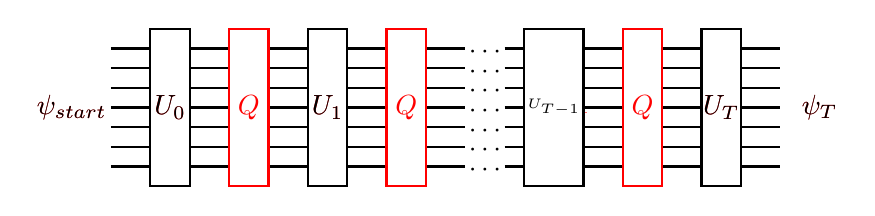
\begin{tikzpicture}[scale=.5]
    \visible<2->{
        \foreach \i in {-1, 1,3,...,15}
            {
                \foreach \j in {0.5, 1, ..., 3.5} {
                        \draw[thick] (\i, \j) -- (\i+1, \j);
                    }
            }

        \foreach \j in {0.5, 1, ..., 3.5} {
                \draw (8.5, \j-.1) node {$\cdots$};
            }}

    \visible<2>{
        \draw[red] (-2, 2) node {$\ket{\psi_{start}}$};
        \draw[red] (17, 2) node {$\ket{\psi_T}$};}

    \visible<3->{
        \draw (-2, 2) node {$\ket{\psi_{start}}$};
        \draw (17, 2) node {$\ket{\psi_T}$};}

    \visible<3>{
        \draw[red,thick] (0,0) -- (1, 0) -- (1, 4) -- (0, 4) -- cycle;
        \draw[red] (.5, 2) node {$U_0$};
        \draw[red,thick] (4,0) -- (5, 0) -- (5, 4) -- (4, 4) -- cycle;
        \draw[red] (4.5, 2) node {$U_1$};
        \draw[red,thick] (10+0,0) -- (10+1, 0) -- (10+1, 4) -- (10+0, 4) -- cycle;
        \draw[red] (10+.5, 2) node {\tiny $U_{T-1}$};
        \draw[red,thick] (10+4,0) -- (10+5, 0) -- (10+5, 4) -- (10+4, 4) -- cycle;
        \draw[red] (10+4.5, 2) node {$U_T$};}
    \visible<4->{
        \draw[thick] (0,0) -- (1, 0) -- (1, 4) -- (0, 4) -- cycle;
        \draw (.5, 2) node {$U_0$};
        \draw[thick] (4,0) -- (5, 0) -- (5, 4) -- (4, 4) -- cycle;
        \draw (4.5, 2) node {$U_1$};
        \draw[thick, fill = white] (10-.5,0) -- (10+1, 0) -- (10+1, 4) -- (10-.5, 4) -- cycle;
        \draw (10+.25, 2) node {\tiny $U_{T-1}$};
        \draw[thick] (10+4,0) -- (10+5, 0) -- (10+5, 4) -- (10+4, 4) -- cycle;
        \draw (10+4.5, 2) node {$U_T$};}
    \visible<4->{
        \draw[red,thick] (2+0,0) -- (2+1, 0) -- (2+1, 4) -- (2+0, 4) -- cycle;
        \draw[red] (2+.5, 2) node {$Q$};
        \draw[red, thick] (2+4,0) -- (2+5, 0) -- (2+5, 4) -- (2+4, 4) -- cycle;
        \draw[red] (2+4.5, 2) node {$Q$};
        \draw[red,thick] (10+2+0,0) -- (10+2+1, 0) -- (10+2+1, 4) -- (10+2+0, 4) -- cycle;
        \draw[red] (10+2+.5, 2) node {$Q$};}


\end{tikzpicture}